\section{Interessentanalyse}
Gruppen vil i dette afsnit undersøge diverse personer/grupper, der kan fungere som interessenter i projektet, altså en person der vil have nytte af eller kan bidrage til projektet. Herefter vil gruppen prioritere disse interessenter, alt efter hvor relevante de er i forhold til projektet.

\textbf{O-løbere} \newline
Den enkelte o-løber vil gerne forbedre sin præstationer. For at kunne dygtiggøre sig er det vigtig at kunne sammenligne detaljeret med andre, lige nu er tiderne mellem hver post (stræktiderne) det eneste der kan sammenlignes og analyseres på. Her er det interessant for løberen at kigge på vejvalg og hastighed mellem posterne, og endda helt ned til de forskellige faser af delstrækkene. \\
Til dette mangler der en mere detaljeret analyse og målbar metode. Problemet håndteres i dag ved at sammenligne skemaer med stræktider og hvis muligt manuelt indtegnede vejvalg på kort efter løberens hukommelse. Der findes nogle apps, gps-ure mm. som kan løse delelementer af problemet, dog er alle disse karakteriseret ved ikke at være særlig brugervenlige og dækker kun delområder eller er meget dyre. Derfor har den enkelte o-løber interesse i dette projekt da produktet vil fokusere på at gøre sammenligning og evaluering af o-løb nemmere og mere effektiv.

\textbf{Træneren}\newline
Træneren vil gerne kunne analysere den enkelte løbers tur detaljeret sammen med løberen og sammenligne med andre løbere. Hvis løberen ikke kan huske hvor vedkommende har løbet eller var faret vild, har træneren svært ved at give sikker og brugbar kritik, da det ikke kan ses på tiderne præcis hvor den enkelte løber har været. Trænere har derfor interesse i et værktøj som kan hjælpe med at evaluere den enkelte løbers tur og sammenligne denne med andre løberes ture, på en detaljeret måde.

\textbf{Løbere}\newline
Fritidsløbere er en interessent i projektet, da det for fritidsløbere kan være interessant at kunne sammenligne sine løbeture med andre, og på den måde kunne bruge det til at forbedre sine tider. 

\textbf{Spejdere}\newline
Spejdere-foreninger der løber orienteringsløb, kan have gavn af projektet, da det kan hjælpe dem med at finde bedre vej, og forbedre deres orientering, ved at de gennem et eventuelt færdigt produkt, kan få hjælp til at se de ruter der er blevet valgt, og hvad der kunne være gjort anderledes. 


\textbf{Tractrac}\newline
TracTrac er et andet produkt, der løser nogle af de samme problemstillingerne, som projektet prøver at løse. De er derfor en interessent i projektet, da projektet kan ende med at blive en konkurrent til deres produkt på nogle punkter. 

\textbf{forbund og foreninger} \newline
O-forbund og foreninger som står for orienteringsløb og medlemmer. Disse kunne være interesseret i projektet, der kunne være til gavn for O-løbere. Måske de kunne bruge et redskab der gør planlægning og administration af ruter lettere.


\subsection{Prioriteringen}
For at prioritere interessenterne i projektet, og finde de vigtigtste interessenter, har gruppen valgt at gøre brug af indlydelse/medvirken-matrixed, som kan ses på figur X herunder.

O-løbere er i dette projektet sat som ressourceperson, da de kan give råd og vejledning til, hvordan deres træning og løb fungere. For at undersøge om der er ting der kan forbedre O-løbernes løb, dette gælder både inden løb, og efter. For så at undersøge om et redskab eller løsning ville være relevant for O-løbere.

Trænere/arrangører er sat som ressourceperson for projektet, da de ligesom O-løberne har et stort indblik i hvordan orienteringsløb fungere, og hvordan det måske kan optimeres eller forbedres. Trænerer/arrangører kan ud over O-løberne, give indblik i hvordan O-løb bliver forberedt.

Orienteringsløbs forbund og foreninger er i dette projekt grå eminence. Da de kan have en indflydelse på projektet, for de kan have nogle opstillede krav og regler til en løsning. Så et fremtidig produkt eller løsning er lovligt for turneringer og O-løb. 

Løbere, spejdere og Tractrac er eksterne i projektet, da hverken deres medvirken eller indflydelse er vigtig for projektet, men projektet kan på en eller anden måde have en indvirkning på dem, enten negativt eller positivt.

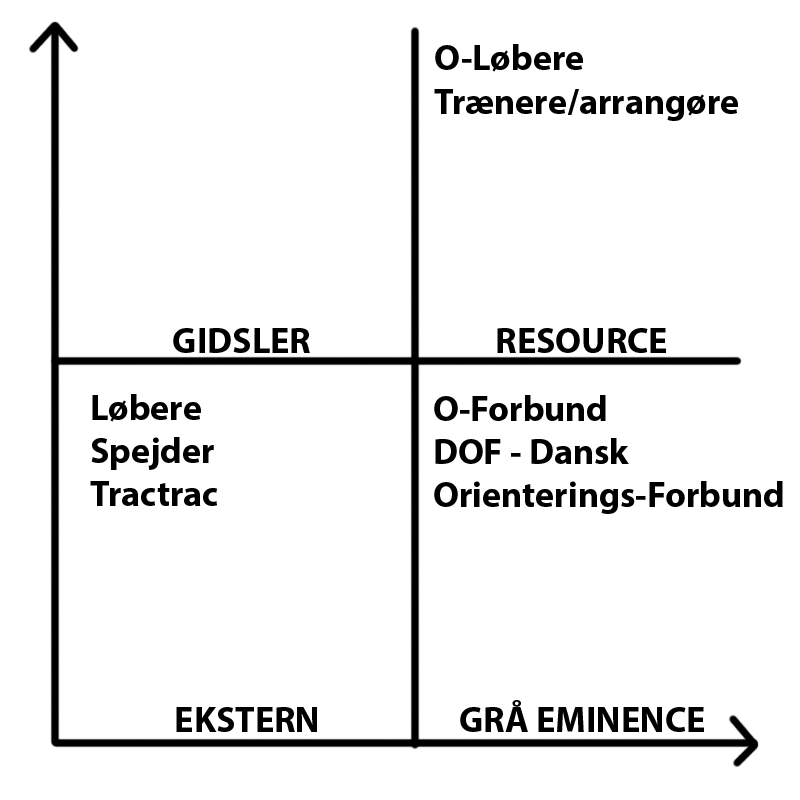
\includegraphics[width=0.90\textwidth]{billeder/Medvirken-indflydelse}
\vspace{4cm}

\subsection{Opsummering}


